\section{RedHat-based distributions (zypper)}
\label{sec:RedHat_zypper}


\subsection{Prerequisites}
The commands described on the following sections require root privileges and Internet connection.

Once the installation process is finished, please log out and back in again to complete the installation. 

\subsection{Package Repository}
To add the package repository you can easily download our predefined lists by executing the following command:
\begin{lstlisting}[language=bash]
x86_64      :  zypper addrepo -f http://compss.bsc.es/repo/rpms/stable/suse/x86_64 compss
noarch      :  zypper addrepo -f http://compss.bsc.es/repo/rpms/stable/suse/noarch compss
\end{lstlisting}

And finally, refresh the repositories:
\begin{lstlisting}[language=bash]
zypper refresh
\end{lstlisting}

\subsection{Installation}
Despite the fact that we recomend users to install the complete COMPSs Framework, we have built different packages to allow users
customize as maximum as possible their installation. Figure \ref{fig:compss_packages_zypper} illustrates the COMPSs packaging structure.
\begin{figure}[ht!]
  \centering
    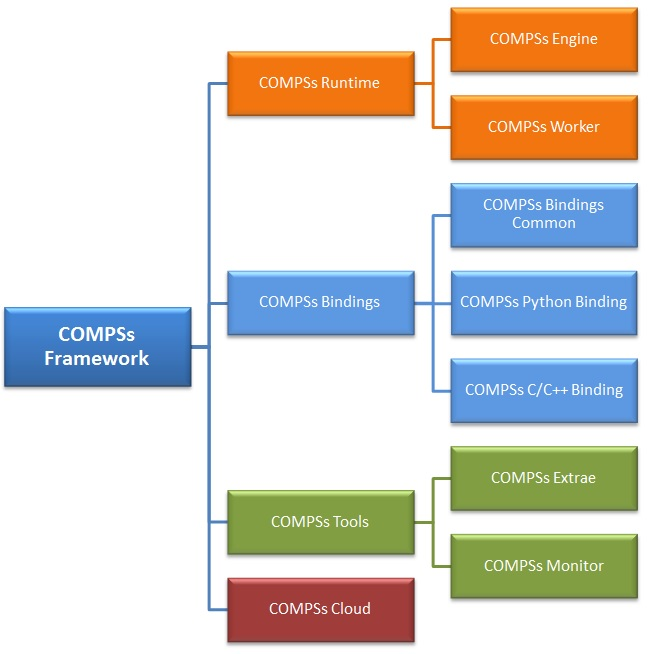
\includegraphics[width=0.75\textwidth]{./Sections/3_RedHat_zypper/Figures/compss_packages.jpeg}
    \caption{COMPSs Packaging structure}
    \label{fig:compss_packages_zypper}
\end{figure}

\newpage
Next we describe the available packages and how to install them. 

\colorComment{If you are willing to have a full COMPSs installation just follow the COMPSs Framework instructions
and skip to next section.}

\begin{itemize}
 \item \textbf{COMPSs Framework} \newline
       Contains the all COMPSs functionalities including the Runtime, all the bindings, all the tools and the cloud connectors.
       \newline
       To install this package please run:
       \begin{lstlisting}[language=bash]
	  zypper install compss-framework
       \end{lstlisting}
 \item \textbf{COMPSs Runtime} \newline
       Contains the COMPSs runtime to support the native functionalities. Install this package if you only need to support Java
       applications.
       \newline
       To install this package please run:
       \begin{lstlisting}[language=bash]
	  zypper install compss-runtime
       \end{lstlisting}
       This package is composed of two sub-packages:
       \begin{itemize}
        \item \textbf{COMPSs Engine} \newline
	      Contains the COMPSs Engine, essential to run COMPSs applications as master.
	      \newline
	      To install this package please run:
	      \begin{lstlisting}[language=bash]
		  zypper install compss-engine
	      \end{lstlisting}
        \item \textbf{COMPSs Worker} \newline
              Contains the minimum installation to allow any machine run as a COMPSs worker.
              \newline
              To install this package please run:
	      \begin{lstlisting}[language=bash]
		  zypper install compss-worker
	      \end{lstlisting}
       \end{itemize}

 \item \textbf{COMPSs Bindings} \newline
       Contains all the bindings to support C/C++ and Python applications. 
       \newline
       To install this package please run:
       \begin{lstlisting}[language=bash]
	  zypper install compss-bindings
       \end{lstlisting}
       This package is composed of three sub-packages:
       \begin{itemize}
        \item \textbf{COMPSs Bindings Common} \newline
	      Contains the API to allow any binding communicate with the COMPSs Runtime. It is necessary for any binding installation.
	      \newline
	      To install this package please run:
	      \begin{lstlisting}[language=bash]
		  zypper install compss-bindings-common
	      \end{lstlisting}
        \item \textbf{COMPSs C/C++ Binding} \newline
	      Contains the C/C++ Binding
	      \newline
	      To install this package please run:
	      \begin{lstlisting}[language=bash]
		  zypper install compss-c-binding
	      \end{lstlisting}
        \item \textbf{COMPSs Python Binding} \newline
	      Contains the Python Binding
	      \newline
	      To install this package please run:
	      \begin{lstlisting}[language=bash]
		  zypper install compss-python-binding
	      \end{lstlisting}
       \end{itemize}

 \item \textbf{COMPSs Tools} \newline
       Contains all the COMPSs Tools.
       \newline
       To install this package please run:
       \begin{lstlisting}[language=bash]
	  zypper install compss-tools
       \end{lstlisting}
       This package is composed of three sub-packages:
       \begin{itemize}
        \item \textbf{COMPSs Extrae} \newline
	      Contains the COMPSs Extrae tool needed to generate and process application traces.
	      \newline
	      To install this package please run:
	      \begin{lstlisting}[language=bash]
		  zypper install compss-extrae
	      \end{lstlisting}
        \item \textbf{COMPSs Monitor} \newline
              Contains the COMPSs Monitor tool needed to monitor the application execution. 
              \newline
	      To install this package please run:
	      \begin{lstlisting}[language=bash]
		  zypper install compss-monitor
	      \end{lstlisting}
       \end{itemize}

 \item \textbf{COMPSs Cloud} \newline
       Contains all the COMPSs Connectors needed to interact with the Cloud.
       \newline
       To install this package please run:
       \begin{lstlisting}[language=bash]
	  zypper install compss-cloud
       \end{lstlisting}
\end{itemize} 

\subsection{Post installation}
Once your COMPSs package has been installed remember to log out and back in again to end the installation process.

If you need to setup your machine for the first time please take a look at Section \ref{sec:Additional_Configuration} for a 
detailed description of the additional configuration. 